\section{Part c}
The model is based upon the study of Ackerman et al. on glucose-insulin regulation, a system of differential equations given by
$$
\frac{d^{2}g}{dt^{2}} + 2\alpha\frac{dg}{dt} + \omega_{0}^{2} = F(t),
$$

whose general solution is
$$
G(t) = G_{0} + Ae^{-\alpha t}cos(\omega(t-\delta)),
$$
where we have five unknown parameters to fit the data:\\

$G_{0}$ represents the equilibrium blood sugar level\\
$\alpha$ measures the ability of system to return to the equilibrium state after being perturbed\\
$\omega$ gives a frequency response to perturbations\\
$A$ gives the amplitude of the response\\
$\delta$ represents a delay in the response.\\

One of the inherent weaknesses of the model is given by the parameter $\alpha$, which was found to give many large errors in the subjects tested by Ackerman et al.; on the other hand, a strength of the model is its resemblance with the damped harmonic oscillator, which is a known system readily analyzed.\\ 
Therefore, we can use a stronger indicator of diabetes given by the natural frequency defined as
$$
\omega_{0} = \omega^{2} + \alpha^{2},
$$
which is used to compute the natural period of the system, given by
$$
T_{0}= \frac{2\pi}{\omega_{0}}.
$$
In this context, this period represents the moment in time at which most of the excess of the glucose ingested has been metabolised and the system has gone back its homeostatic conditions. We know from literature that\\

if $T_{0} < 4 \rightarrow$ Non-diabetic subject;\\
if $T_{0} > 4 \rightarrow$ Diabetic subject.\\

After running a best fit to the data given, we found that for the two subjects we have two different natural frequencies of respectively:\\

First Subject = $G_{1} \longrightarrow \omega_{0} \approx 1.903 hrs^{-1}$\\
Second Subject = $G_{2} \longrightarrow \omega_{0} \approx 1.279 hrs^{-1}$,\\

which give the following natural periods:\\

$G_{1} \longrightarrow T_{0} \approx 3.30 hrs < 4 \rightarrow$ Non-diabetic \\
$G_{2} \longrightarrow T_{0} \approx 4.9 hrs > 4 \rightarrow$ Diabetic.\\

So we found a difference of about 33\% between the two natural frequencies as well as between the two natural periods. And the situation can be visualised properly by graphing the two models along with the data given.

\begin{figure}[H]
	\centering
	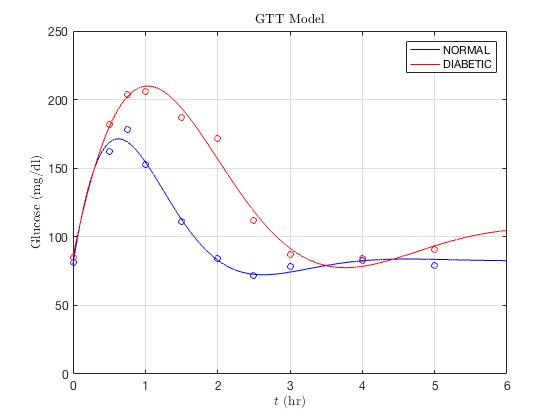
\includegraphics[scale=0.6]{DIABETES_Prob1.jpg}
	\caption{Alckerman model data-fitting}
\end{figure}

From the graph in Fig.1.1 we can see that the model fits the data really well, especially for the non-diabetic case (blu line in the graph). In fact, its Sum of Square Errors was found to be
$$
SSE_{Non-diabetic} \approx 165.7,
$$ 
whereas for the diabetic case we see some incongruences between the model and data, as it is confirmed by its SSE, found to be
$$
SSE_{Diabetic} \approx 406.33.
$$
For the non-diabetic case, we see a steady increase in the glucose level in the blood from its starting point of $G(0) = 81 mg/dL$ to its maximum found at $t \approx 0.7hrs$, so around 42 minutes after the ingestion of a large amount of glucose, to be around $G_{max}=170mg/dL$. Looking at the graph, we see that the model actually underestimates the maximum given by the data found at $t=0.75$ to be $G_{max}=178mg/dL$. Then the model fits the data almost perfectly and seems to level off after 4 hours, and at $t=4hrs$ the data from the non-diabetic subject and the diabetic subject overlap.\\
As for the diabetic case (red line in the figure), the graph fits the data reasonably well, even though it seems to be less accurate than the non-diabetic case (but it still seems to be within the margin of error). The model overestimates the maximum concentration of glucose in the blood, accurately found at $t=1hr$, therefore one hour after the ingestion of glucose, but it appears to be a value slightly greater than the $206mg/mL$ given from the data. According to the model, the level of glucose in the blood steadily increases to its maximum and then decreases to its minimum at around $t=3.7hrs$, or 3 hours and 42 minutes after the ingestion of glucose, and then increases again and appears to level off after six hours, but at a value much higher (over 100mg of glucose per dL of blood) than pre-fasting conditions.\\
The two models intersect at $t \approx 3.50$ and $t \approx 4.43$, i.e. approximately after three hours and thirty minutes and after four hours and twenty-six minutes from the ingestion of glucose. At those points the concentration of glucose in the blood is, respectively, 79mg/dL and 83.7mg/dL, and it's obviously the same for both subjects. At $t \approx 3.50$, according to the model, the non-diabetic subject sees a slight increase in the glucose level in the blood, which indeed happens according to the data given, but then it levels off after fours hours, going back to homeostatic conditions.\\
Whereas, for the diabetic subject, the model steadily decreases before the intersection point at $t \approx 3.50$, then it appears to have an interflection point immediately after and starts to steadily increase. They intersect again at $t \approx 4.43$, but, while the glucose level for the non-diabetic subject levels off, the diabetic subject sees a steady increase in the glucose concentration in the blood up until six hours after fasting, according to the model.
\\
According to a famous diabetologist, the blood glucose concentration of a non-diabetic who has just absorbed a large amount of glucose will be at or below fasting level in 2 hours or less. Using this criteria to analyse our model, we see that in fact the non-diabetic subject has a concentration of glucose in the blood of 81mg/dL before fasting; after two hours the glucose level in his/her blood is 84mg/dL, which is very close to the pre-fasting value. The level continues to drop for more than one hour after that (it's 78mg/dL at $t=3hrs$) and then increases back to 83mg/dL at $t=4hrs$. Then it decreases again, it's 79mg/dL at $t=5hrs$, and according to our model it levels off after that, indicating that all the glucose should have been absorbed.\\
For the diabetic subject we have a very different situation. Even though the two subjects start with a pretty similar pre-fasting level of glucose, 81 mg/dL for the non-diabetic case and 85mg/dL for the diabetic case, which is a difference of less than 5\%, after two hours the diabetic subject has a level of glucose in his/her blood of 172mg/dL, against the 84mg/dL of the non-diabetic case, a difference of almost 52\% between the two cases.\\
In fact, in order to go back to his/her pre-fasting level of glucose, the diabetic subject has to wait more than three hours (at $t=3hrs$ his/her level is at 87mg/dL), as we see that at $t=4hrs$ the glucose concentration is 84mg/dL. However, after that point, the glucose level seems to be increasing again as it is found to be 91mg/dL after five hours and, according to our model, seems to increase even after that point, which indicates that some therapy has to be performed on the subject in order to regulate his/her level of glucose in the blood from keeping to increase steadily.\\
Using the Oral Glucose Tolerance Test (OGTT) to analyse our data, we see that the fasting level of both subjects are below 100mg/dL and therefore, according to this standard test, both subject would be considered non-diabetic at $t=0$.\\
However, as we continue our analysis, we see that at $t=1$ the situation is quite different. In fact, the first subject has a glucose level in his/her blood of 153mg/dL, which is considered normal as it is below 180mg/dL, whereas the second subject has a glucose level in his/her blood of 206mg/dL, which is considered diabetic.\\
At $t=2$ the test suggests that non-diabetic individuals have glucose level below 140mg/dL, whereas diabetic individuals have glucose level above 180mg/dL. For our case, the first subject has glucose level of 84mg/dL after two hours from fasting, which indicates non-diabetic conditions according to the OGTT. Yet, the second subject has glucose level of 172mg/dL at $t=2$, which is way above normal conditions, but still below the value of 200mg/dL, which is considered diabetic.\\
Thus, the OGTT does not seem to be a good way for testing diabetes, as it is found to be erroneous for both  $t=0$ and $t=2$, whereas the Alkerman model represents a very good fit for the data and seems to be a better way to test diabetic conditions in individuals.